\section{Short-term Personalized Multi-Modal Interactions}

One of the main goals of the COACHES project is personalized short-term interactions with non-expert users, that are typical customers of a shopping mall.

Short-term ...

Personalized ...

Multi-modal interaction ...



\begin{figure}
\centering
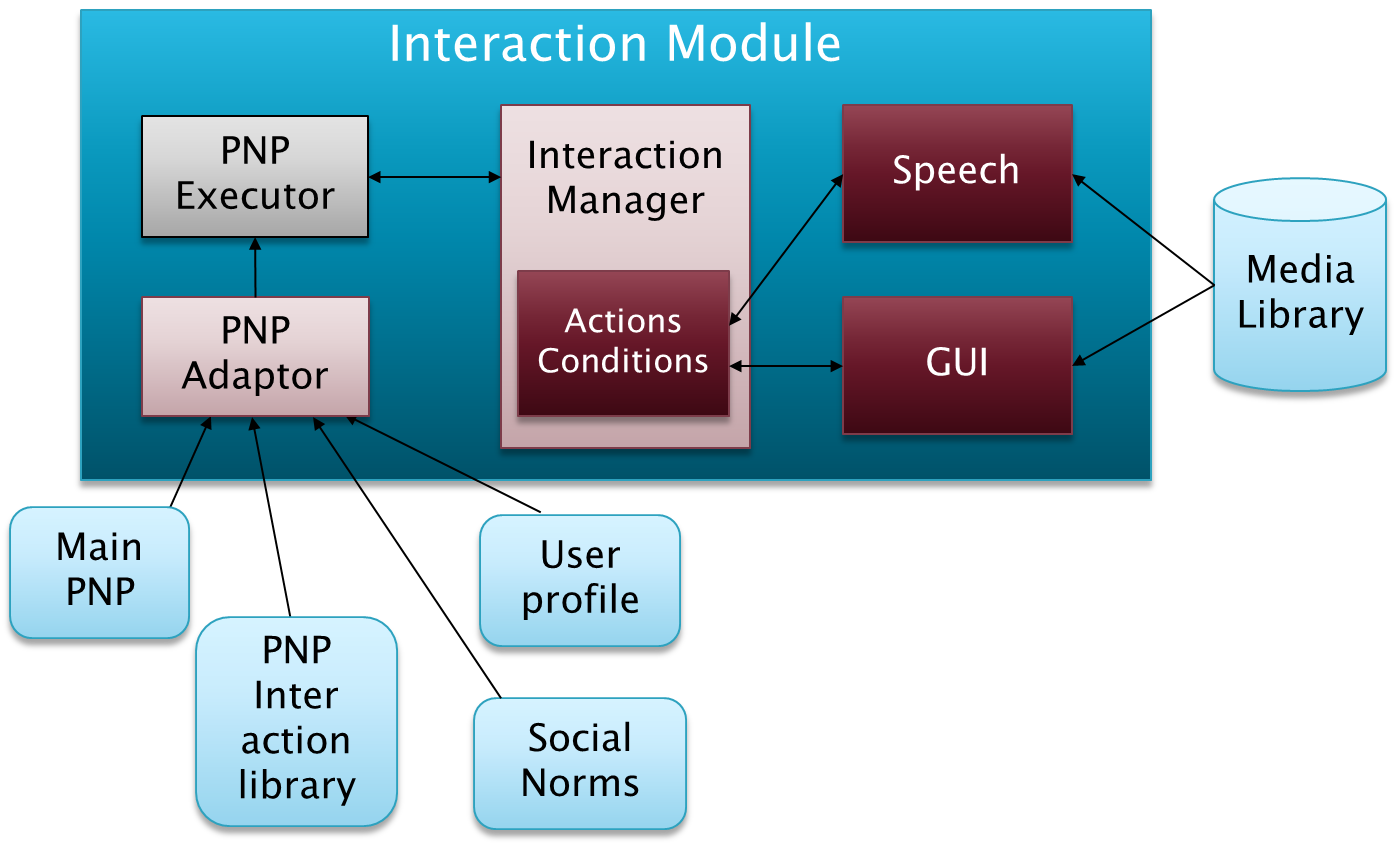
\includegraphics[width=0.95\textwidth]{fig/WP3.png}
\caption{Architecture of the Human-Robot Interaction sub-system.}
\label{fig:swarch}
\end{figure}

The architecture of the Human-Robot Interaction sub-system is illustrated in Figure \ref{fig:swarch} and their components are described in the following.

\subsection{Interaction Manager}
% Description of the Interaction Manager component...

The interactions are coordinated by an Interaction Manager (IM), which is a complex component that integrates different information produced by other components or available in the system and controls the interaction with a user.

The IM actually coordinates all the robot modules (both the ones related with human-robot interaction and the ones used for implementing the basic robotic functionalities).
Its goal is thus to provide effective robot behaviors, including the personalized short-term multi-modal interactions.

The IM module takes as input: a goal-oriented plan, the user profile, a set of general social norms and a media library. The plan and the user profile dynamically change over time, depending on the current situation the robot is facing, while the social rules and the media library are stored before the start of the robot task.

The IM module is within the framework of the Petri Net Plans (PNP) formalism \cite{}. More specifically, the IM is the action and condition server that executes actions and provides conditions, according to the requests of the PNP Executor module.
A main plan, which include \emph{interaction plans} for HRI behaviors, is then executed by the PNP Executor, that is a general-purpose process that calls actions and receives conditions to/from the IM module.
In this way, we can easily separate the implementation of the basic actions and conditions (that are implemented in the HRI module) from their composition (that is implemented through PNP). 


PNP are based on two main concepts: \emph{actions} (i.e., output operations) and \emph{conditions} (i.e., input operations). Actions include motion of the robot in the environment, spoken sentences issued by the on-board speakers, text, images, videos or animations shown on the on-board screen, etc.
Conditions include the result of perception routines (e.g., image processing or speech recognition), the input given by a user through a GUI on the on-board screen, information about personal data of user acquired through a reader of fidelity cards, etc.

The use of PNP for representing in an integrated way all these different kinds of actions and conditions allows for a strong coordination between the different sub-systems of the robot and for showing more complex behaviors and, in particular, a multi-modal interaction that can be easily customized according to the user.



\subsection{Speech and GUI modules}

The interaction modalities considered so far in the project are speech and graphical interfaces.

These interaction sub-systems that are described in the next sections are: 1) speech sub-system, that enables the robot with voice interactions with users, 2) GUI sub-system, that allows for interaction through a graphical interface, ???


\paragraph{Speech recognition and synthesis.}
The speech module allows the robot to communicate with humans through vocal interactions. 
It  is formed by two components: Automatic Speech Recognition (ASR) and Text-To-Speech (TTS),.

The ASR component analyzes audio data coming from a microphone and extract semantic information about the spoken sentences, according to a predefined grammar. This component allows the robot to understand user spoken commands.
The speech recognition module is based on the Microsoft engine and on a further processing module that builds the semantic frames of the recognized sentences.
More details on the approach are available in \cite{Ba...}.

The TTS component transforms text messages in audio data that are then emitted by the speakers on-board the robot. This enables the robot to speak to people. The Microsoft TTS engine is used for this module.


\paragraph{Graphical User Interface}


The GUI component implements a graphical input and output interface between users and robots that is displayed through the touch screen on-board the robot. The GUI defines actions (i.e., output operations) and conditions (i.e., input operations) that are integrated in the IM with other communication primitives (e.g., speech) in order to implement a multi-modal interaction.

\vspace{1cm}

The Speech and GUI components make available to the IM the implementation of actions and conditions that are executed according to the PNPs. These are summarized in the following table.

\vspace{1em}
\begin{center}
%\begin{table}
\begin{tabular}{|c|c|c|} \hline
 & {\bf Action} & {\bf Condition} \\  \hline
Speech & 
\begin{tabular}{c}
\emph{Say} \\ 
speak information though TTS
\end{tabular} & 
\begin{tabular}{c}
\emph{ASR} \\ 
Results of ASR
\end{tabular} \\ \hline
GUI & 
\begin{tabular}{c}
\emph{Show} \\ 
show information on the GUI
\end{tabular} & 
\begin{tabular}{c}
\emph{GUI} \\ 
Results of GUI input
\end{tabular} \\ \hline
\end{tabular}  
%\label{}
%\caption
\end{center}
\vspace{1em}


